We initially approached the problem of chess-pieces object detection using DETR (Detection Transformer), with a ResNet-50 backbone, used for object detection tasks.
The DETR model was pre-trained on the COCO dataset and fine-tuned on a custom dataset of 2000 chess images, which included various chess pieces in different lighting conditions,
 angles, and designs annotated in the COCO format with 12 classes representing the different chess pieces (e.g., white-pawn, white-knight, white-bishop, etc.).
However, we encountered several challenges with this method, particularly in terms of performance and accuracy.
Despite tuning and training the model for 100, 150 and 200 epoch, DETR consistently underperformed.
The DETR model struggled with the variability of chess pieces in different lighting conditions, angles, and designs, leading to suboptimal detection results.
We found out that the model was not able to converge properly, and the loss function did not decrease as expected during training.
This led us to explore alternative approaches for chess-piece object detection.

We then turned our attention to YOLOv8, a state-of-the-art object detection model that has shown promising results in various applications.
We trained YOLOv8 on the same custom dataset of 2000 chess images, which included various chess pieces in different lighting conditions, angles, and designs.
The training process was more successful with YOLOv8, as the model was able to converge properly and achieve a lower loss function.
The YOLOv8 model demonstrated superior performance in terms of accuracy and robustness compared to DETR.

The model was trained from a pre-trained checkpoint found online and fine-tuned on our custom dataset.[ref to github repo]
We conducted three training runs with different parameters like:
\begin{itemize}
    \item Data augmentations (mosaic augmentation)
    \item HSV shifts
    \item Horizontal and vertical flips
\end{itemize}
The training was performed using PyTorch 2.1 on an NVIDIA RTX 3090 GPU with 24GB of VRAM.

The three training runs were conducted with the two datasets in this order:
\begin{itemize}
    \item YOLOv8m run 1: A small dataset found on Roboflow, which contains 100 images of chess pieces in different lighting conditions and angles.
    \item YOLOv8m run 2: ChessRed2K dataset, which contains 2000 images of chess pieces in various conditions.
    \item YOLOv8m run 3: Starting from run 1 we used ChessRed2K dataset for finetuning the model.
\end{itemize}

The YOLOv8m model performed well, achieving a mean Average Precision (mAP) of
 approximately 0.87 at IoU threshold 0.5 and a
  mAP of approximately 0.77 at IoU thresholds from 0.5 to 0.95.

As we can see in the table below, the model achieved high precision
 and recall values across the three training runs,
indicating its effectiveness in detecting and classifying chess pieces.
All the runs showed converged approximately in 200 epochs.

\begin{table}[ht]
\centering
\caption{Key performance metrics for the three YOLOv8m training runs.}
\label{tab:YOLOv8-results}
\resizebox{\linewidth}{!}{%
\begin{tabular}{lccccl}
\toprule
\textbf{Run} & \textbf{Precision (B)} & \textbf{Recall (B)} & \textbf{mAP@0.5} & \textbf{mAP@0.5:0.95} \\
\midrule
YOLOv8m Run 1 & $\sim$0.88 & $\sim$0.93 & $\sim$0.87 & $\sim$0.75 \\
YOLOv8m Run 2 & $\sim$0.90 & $\sim$0.95 & $\sim$0.89 & $\sim$0.78 \\
YOLOv8m Run 3 & $\sim$0.87 & $\sim$0.91 & $\sim$0.85 & $\sim$0.72 \\
\bottomrule
\end{tabular}
}
\end{table}


In terms of loss behavior, we decided to use three different loss functions:
\begin{itemize}
    \item Classification Loss: it measures the accuracy of the model predictions in classfiying the class inside the bounding box.
    For this loss YOLOv8m uses a binary cross-entropy loss function.
    \item Box Loss: it measures the accuracy of the model in predicting bounding box positions and sizes. It's calculated with a combinantion of IoU (Interection over Union).
    \item Distribution Focal Loss: this loss function is an advanced feature of YOLOv8. It measures the accuracy of the model in identifying the presence of objects inside the image. It's used to handle better small objects.
\end{itemize}

\begin{table}[ht]
\centering
\caption{Final loss values for the three YOLOv8m runs. All values are approximate and taken at convergence (step $\sim$200).}
\label{tab:yolov8-loss}
\resizebox{\linewidth}{!}{%
\begin{tabular}{lccc}
\toprule
\textbf{Run} & \textbf{Classification Loss (cls\_loss)} & \textbf{Box Loss (box\_loss)} & \textbf{DFL Loss (dfl\_loss)} \\
\midrule
YOLOv8m Run 1 & $\sim$0.06 & $\sim$0.35 & $\sim$1.10 \\
YOLOv8m Run 2 & $\sim$0.05 & $\sim$0.32 & $\sim$1.05 \\
YOLOv8m Run 3 & $\sim$0.07 & $\sim$0.38 & $\sim$1.15 \\
\bottomrule
\end{tabular}
}
\end{table}

Compared to earlier training runs and attempts with DETR that showed high loss values and poor convergence, YOLOv8m performed significantly better in terms of loss values and detection robustness.
We decided to use the third run of YOLOv8m as our final model for chess-piece object detection, as it showed the best performance in terms of precision, recall, and mAP values.

\begin{figure}[ht]
\centering
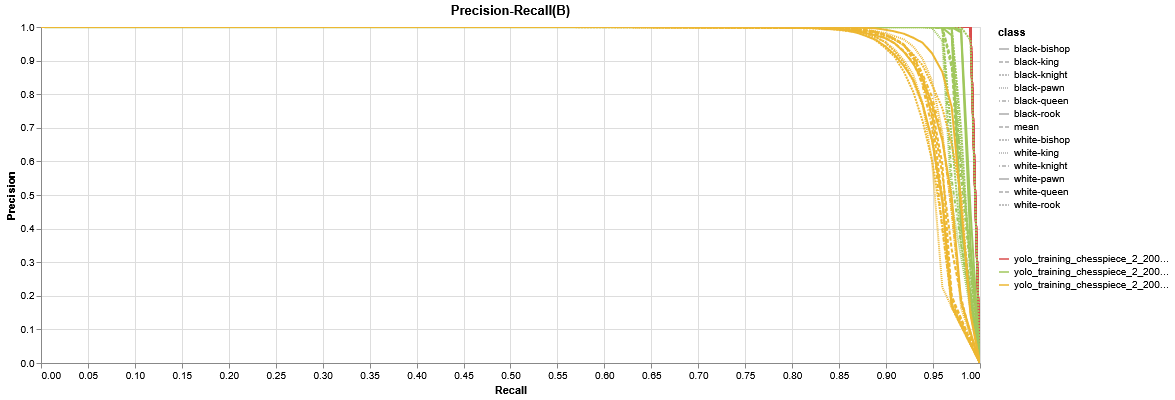
\includegraphics[width=\linewidth]{images/PR-runs-obj.png}
\caption{Precision-Recall curve for YOLOv8m. Yellow: Run 1, Green: Run 2, Red: Run 3. }
\label{fig:chess-detection}
\end{figure}
